\documentclass[12pt, a4paper,  BCOR=8.25mm, DIV=15]{scrartcl}\usepackage[]{graphicx}\usepackage[]{color}
%% maxwidth is the original width if it is less than linewidth
%% otherwise use linewidth (to make sure the graphics do not exceed the margin)
\makeatletter
\def\maxwidth{ %
  \ifdim\Gin@nat@width>\linewidth
    \linewidth
  \else
    \Gin@nat@width
  \fi
}
\makeatother

\definecolor{fgcolor}{rgb}{0.345, 0.345, 0.345}
\newcommand{\hlnum}[1]{\textcolor[rgb]{0.686,0.059,0.569}{#1}}%
\newcommand{\hlstr}[1]{\textcolor[rgb]{0.192,0.494,0.8}{#1}}%
\newcommand{\hlcom}[1]{\textcolor[rgb]{0.678,0.584,0.686}{\textit{#1}}}%
\newcommand{\hlopt}[1]{\textcolor[rgb]{0,0,0}{#1}}%
\newcommand{\hlstd}[1]{\textcolor[rgb]{0.345,0.345,0.345}{#1}}%
\newcommand{\hlkwa}[1]{\textcolor[rgb]{0.161,0.373,0.58}{\textbf{#1}}}%
\newcommand{\hlkwb}[1]{\textcolor[rgb]{0.69,0.353,0.396}{#1}}%
\newcommand{\hlkwc}[1]{\textcolor[rgb]{0.333,0.667,0.333}{#1}}%
\newcommand{\hlkwd}[1]{\textcolor[rgb]{0.737,0.353,0.396}{\textbf{#1}}}%

\usepackage{framed}
\makeatletter
\newenvironment{kframe}{%
 \def\at@end@of@kframe{}%
 \ifinner\ifhmode%
  \def\at@end@of@kframe{\end{minipage}}%
  \begin{minipage}{\columnwidth}%
 \fi\fi%
 \def\FrameCommand##1{\hskip\@totalleftmargin \hskip-\fboxsep
 \colorbox{shadecolor}{##1}\hskip-\fboxsep
     % There is no \\@totalrightmargin, so:
     \hskip-\linewidth \hskip-\@totalleftmargin \hskip\columnwidth}%
 \MakeFramed {\advance\hsize-\width
   \@totalleftmargin\z@ \linewidth\hsize
   \@setminipage}}%
 {\par\unskip\endMakeFramed%
 \at@end@of@kframe}
\makeatother

\definecolor{shadecolor}{rgb}{.97, .97, .97}
\definecolor{messagecolor}{rgb}{0, 0, 0}
\definecolor{warningcolor}{rgb}{1, 0, 1}
\definecolor{errorcolor}{rgb}{1, 0, 0}
\newenvironment{knitrout}{}{} % an empty environment to be redefined in TeX

\usepackage{alltt}
\usepackage[utf8]{inputenc}
\usepackage{newfloat}
\DeclareFloatingEnvironment[name={Supplementary Figure}]{suppfigure}

\newenvironment{itemizz}%
  {\begin{itemize}%
    \setlength{\itemsep}{2pt}%
    \setlength{\parskip}{2pt}}%
  {\end{itemize}}

\newcommand{\txtt}[1]{{\texttt{#1}}}
\IfFileExists{upquote.sty}{\usepackage{upquote}}{}
\begin{document}
%\VignetteEngine{knitr::knitr}
%\VignetteIndexEntry{Graphics (Set 9)}



\title{9: Graphics}
\author{John H Maindonald}
\maketitle

\vspace*{-1cm}

\begin{knitrout}
\definecolor{shadecolor}{rgb}{0.969, 0.969, 0.969}\color{fgcolor}\begin{kframe}
\begin{alltt}
\hlstd{doFigs} \hlkwb{<-} \hlnum{TRUE}
\end{alltt}
\end{kframe}
\end{knitrout}

\begin{knitrout}
\definecolor{shadecolor}{rgb}{0.969, 0.969, 0.969}\color{fgcolor}\begin{kframe}
\begin{alltt}
\hlstd{fig9.1} \hlkwb{<-} \hlkwa{function}\hlstd{()\{}
\hlcom{## ---- brain-body ----}
\hlkwd{plot}\hlstd{(Brainwt} \hlopt{~} \hlstd{Bodywt,} \hlkwc{xlim}\hlstd{=}\hlkwd{c}\hlstd{(}\hlnum{0}\hlstd{,} \hlnum{300}\hlstd{),}
     \hlkwc{ylim}\hlstd{=}\hlkwd{c}\hlstd{(}\hlnum{0}\hlstd{,}\hlnum{1500}\hlstd{),} \hlkwc{data}\hlstd{=primates,}
     \hlkwc{xlab}\hlstd{=}\hlstr{"Body weight (kg)"}\hlstd{,}
     \hlkwc{ylab}\hlstd{=}\hlstr{"Brain weight (g)"}\hlstd{)}
\hlcom{# Specify xlim to allow room for the labels}
\hlkwd{with}\hlstd{(primates,}
     \hlkwd{text}\hlstd{(Brainwt} \hlopt{~} \hlstd{Bodywt,}
          \hlkwc{labels}\hlstd{=}\hlkwd{rownames}\hlstd{(primates),} \hlkwc{pos}\hlstd{=}\hlnum{4}\hlstd{))}
\hlcom{# pos: pos=1 (below), 2 (left), 3 (above)}
\hlstd{\}}
\end{alltt}
\end{kframe}
\end{knitrout}

\begin{knitrout}
\definecolor{shadecolor}{rgb}{0.969, 0.969, 0.969}\color{fgcolor}\begin{kframe}
\begin{alltt}
\hlstd{supp9.1} \hlkwb{<-} \hlkwa{function}\hlstd{()\{}
\hlkwa{if}\hlstd{(}\hlopt{!}\hlkwd{require}\hlstd{(RColorBrewer))}\hlkwd{stop}\hlstd{(}\hlstr{"RColorBrewer must be installed"}\hlstd{)}
\hlcom{## ---- col-plots ----}
\hlstd{opt} \hlkwb{<-} \hlkwd{options}\hlstd{(}\hlkwc{width}\hlstd{=}\hlnum{75}\hlstd{)}
\hlstd{colpal} \hlkwb{<-} \hlkwd{rev}\hlstd{(}\hlkwd{list}\hlstd{(}
    \hlstr{"Default palette"} \hlstd{=} \hlkwd{palette}\hlstd{()[}\hlnum{1}\hlopt{:}\hlnum{8}\hlstd{],}  \hlkwc{cm.colors} \hlstd{=} \hlkwd{cm.colors}\hlstd{(}\hlnum{12}\hlstd{),}
    \hlkwc{terrain.colors} \hlstd{=} \hlkwd{terrain.colors}\hlstd{(}\hlnum{12}\hlstd{),} \hlkwc{heat.colors} \hlstd{=} \hlkwd{heat.colors}\hlstd{(}\hlnum{12}\hlstd{),}
    \hlkwc{blueRamp} \hlstd{=} \hlkwd{colorRampPalette}\hlstd{(}\hlkwd{c}\hlstd{(blues9,} \hlstr{"white"}\hlstd{))(}\hlnum{12}\hlstd{),}
    \hlstr{"Brewer-Set1"} \hlstd{=} \hlkwd{brewer.pal}\hlstd{(}\hlnum{8}\hlstd{,} \hlstr{"Set1"}\hlstd{),}
    \hlstr{"Brewer-Dark2"} \hlstd{=} \hlkwd{brewer.pal}\hlstd{(}\hlnum{8}\hlstd{,} \hlstr{"Dark2"}\hlstd{)))}
\hlstd{palnam} \hlkwb{<-} \hlkwd{names}\hlstd{(colpal)}
\hlkwd{plot}\hlstd{(}\hlnum{1}\hlstd{,} \hlnum{1}\hlstd{,} \hlkwc{xlim}\hlstd{=}\hlkwd{c}\hlstd{(}\hlnum{0.5}\hlstd{,}\hlnum{12.5}\hlstd{),} \hlkwc{ylim}\hlstd{=}\hlkwd{c}\hlstd{(}\hlnum{0}\hlstd{,}\hlkwd{length}\hlstd{(palnam)}\hlopt{+}\hlnum{0.5}\hlstd{),} \hlkwc{type}\hlstd{=}\hlstr{"n"}\hlstd{,}
     \hlkwc{axes}\hlstd{=}\hlnum{FALSE}\hlstd{,} \hlkwc{xlab}\hlstd{=}\hlstr{""}\hlstd{,} \hlkwc{ylab}\hlstd{=}\hlstr{""}\hlstd{)}
\hlkwa{for}\hlstd{(i} \hlkwa{in} \hlnum{1}\hlopt{:}\hlkwd{length}\hlstd{(palnam))\{}
    \hlstd{len} \hlkwb{<-} \hlkwd{length}\hlstd{(colpal[[i]])}
    \hlkwd{points}\hlstd{(}\hlnum{1}\hlopt{:}\hlstd{len,} \hlkwd{rep}\hlstd{(i,len),} \hlkwc{pch}\hlstd{=}\hlnum{15}\hlstd{,} \hlkwc{col}\hlstd{=colpal[[i]],} \hlkwc{cex}\hlstd{=}\hlnum{5.5}\hlstd{)}
    \hlkwd{legend}\hlstd{(}\hlnum{1}\hlstd{, i}\hlopt{+}\hlnum{0.025}\hlstd{, palnam[i],} \hlkwc{adj}\hlstd{=}\hlnum{0}\hlstd{,} \hlkwc{box.col}\hlstd{=}\hlstr{"white"}\hlstd{,} \hlkwc{bg}\hlstd{=}\hlstr{"white"}\hlstd{,}
           \hlkwc{x.intersp}\hlstd{=}\hlnum{0}\hlstd{,} \hlkwc{y.intersp}\hlstd{=}\hlnum{0}\hlstd{,} \hlkwc{yjust}\hlstd{=}\hlnum{0}\hlstd{)}
\hlstd{\}}
\hlkwd{options}\hlstd{(opt)}
\hlstd{\}}
\end{alltt}
\end{kframe}
\end{knitrout}

\begin{knitrout}
\definecolor{shadecolor}{rgb}{0.969, 0.969, 0.969}\color{fgcolor}\begin{kframe}
\begin{alltt}
\hlstd{fig9.2} \hlkwb{<-} \hlkwa{function}\hlstd{()\{}
\hlcom{## ---- alpha-ex ----}
\hlcom{## Sample from the 15992 rows}
\hlstd{dfsamp} \hlkwb{<-} \hlstd{cps1[}\hlkwd{sample}\hlstd{(}\hlkwd{nrow}\hlstd{(cps1),} \hlnum{3000}\hlstd{), ]}
\hlkwd{plot}\hlstd{(re78} \hlopt{~} \hlstd{re75,} \hlkwc{data}\hlstd{=dfsamp,} \hlkwc{pch}\hlstd{=}\hlnum{20}\hlstd{,} \hlkwc{cex}\hlstd{=}\hlnum{0.5}\hlstd{,}
     \hlkwc{col}\hlstd{=}\hlstr{"black"}\hlstd{)}
\hlkwd{mtext}\hlstd{(}\hlkwc{side}\hlstd{=}\hlnum{3}\hlstd{,} \hlkwc{line}\hlstd{=}\hlnum{0.5}\hlstd{,} \hlstr{"A: 100% opacity"}\hlstd{,} \hlkwc{adj}\hlstd{=}\hlnum{0}\hlstd{)}
\hlkwd{plot}\hlstd{(re78} \hlopt{~} \hlstd{re75,} \hlkwc{data}\hlstd{=dfsamp,} \hlkwc{pch}\hlstd{=}\hlnum{20}\hlstd{,} \hlkwc{cex}\hlstd{=}\hlnum{0.5}\hlstd{,}
     \hlkwc{col}\hlstd{=}\hlkwd{adjustcolor}\hlstd{(}\hlstr{"black"}\hlstd{,} \hlkwc{alpha}\hlstd{=}\hlnum{0.4}\hlstd{))}
\hlkwd{mtext}\hlstd{(}\hlkwc{side}\hlstd{=}\hlnum{3}\hlstd{,} \hlkwc{line}\hlstd{=}\hlnum{0.5}\hlstd{,} \hlstr{"B: 40% opacity"}\hlstd{,} \hlkwc{adj}\hlstd{=}\hlnum{0}\hlstd{)}
\hlstd{blueRamp} \hlkwb{<-} \hlkwd{colorRampPalette}\hlstd{(}\hlkwd{c}\hlstd{(}\hlstr{"white"}\hlstd{, blues9))}
\hlkwd{with}\hlstd{(dfsamp,} \hlkwd{smoothScatter}\hlstd{(re75}\hlopt{~}\hlstd{re74,}
                           \hlkwc{colramp}\hlstd{=blueRamp))}
\hlkwd{mtext}\hlstd{(}\hlkwc{side}\hlstd{=}\hlnum{3}\hlstd{,} \hlkwc{line}\hlstd{=}\hlnum{0.5}\hlstd{,} \hlstr{"C: Color density plot"}\hlstd{,}
      \hlkwc{adj}\hlstd{=}\hlnum{0}\hlstd{)}
\hlstd{\}}
\end{alltt}
\end{kframe}
\end{knitrout}

\begin{knitrout}
\definecolor{shadecolor}{rgb}{0.969, 0.969, 0.969}\color{fgcolor}\begin{kframe}
\begin{alltt}
\hlstd{fig9.3} \hlkwb{<-} \hlkwa{function}\hlstd{()\{}
\hlcom{## ---- aspect ----}
\hlkwd{plot}\hlstd{((}\hlnum{1}\hlopt{:}\hlnum{30}\hlstd{)}\hlopt{*}\hlnum{0.92}\hlstd{,} \hlkwd{sin}\hlstd{((}\hlnum{1}\hlopt{:}\hlnum{30}\hlstd{)}\hlopt{*}\hlnum{0.92}\hlstd{),}
     \hlkwc{xlab}\hlstd{=}\hlstr{""}\hlstd{,} \hlkwc{ylab}\hlstd{=}\hlstr{""}\hlstd{)}
\hlstd{\}}
\end{alltt}
\end{kframe}
\end{knitrout}

\begin{knitrout}
\definecolor{shadecolor}{rgb}{0.969, 0.969, 0.969}\color{fgcolor}\begin{kframe}
\begin{alltt}
\hlstd{supp9.2} \hlkwb{<-} \hlkwa{function}\hlstd{()\{}
\hlcom{## ---- Animals-body-brain ----}
\hlcom{## Supplementary figure 9.2}
\hlkwd{library}\hlstd{(MASS)}
\hlstd{oldpar} \hlkwb{<-} \hlkwd{par}\hlstd{(}\hlkwc{pch}\hlstd{=}\hlnum{16}\hlstd{,} \hlkwc{pty}\hlstd{=}\hlstr{"s"}\hlstd{,} \hlkwc{mfrow}\hlstd{=}\hlkwd{c}\hlstd{(}\hlnum{2}\hlstd{,}\hlnum{2}\hlstd{))}
\hlkwd{with}\hlstd{(Animals, \{}      \hlcom{# bracket several R statements}
  \hlkwd{plot}\hlstd{(body, brain)}
  \hlkwd{plot}\hlstd{(}\hlkwd{sqrt}\hlstd{(body),} \hlkwd{sqrt}\hlstd{(brain))}
  \hlkwd{plot}\hlstd{(body}\hlopt{^}\hlnum{0.1}\hlstd{, brain}\hlopt{^}\hlnum{0.1}\hlstd{)}
  \hlkwd{plot}\hlstd{(}\hlkwd{log}\hlstd{(body),} \hlkwd{log}\hlstd{(brain))}
\hlstd{\})}                   \hlcom{# close both sets of brackets}
\hlkwd{par}\hlstd{(oldpar)}          \hlcom{# Restore former settings}
\hlstd{\}}
\end{alltt}
\end{kframe}
\end{knitrout}

\begin{knitrout}
\definecolor{shadecolor}{rgb}{0.969, 0.969, 0.969}\color{fgcolor}\begin{kframe}
\begin{alltt}
\hlstd{fig9.4} \hlkwb{<-} \hlkwa{function}\hlstd{()\{}
\hlcom{## ---- poss-hist ----}
\hlstd{ftotlen} \hlkwb{<-} \hlkwd{subset}\hlstd{(possum, sex}\hlopt{==}\hlstr{"f"}\hlstd{)[,} \hlstr{"totlngth"}\hlstd{]}
\hlcom{## Left panel: breaks at 72.5, 77.5,..}
\hlkwd{hist}\hlstd{(ftotlen,} \hlkwc{breaks} \hlstd{=} \hlnum{72.5} \hlopt{+} \hlstd{(}\hlnum{0}\hlopt{:}\hlnum{5}\hlstd{)}\hlopt{*}\hlnum{5}\hlstd{,} \hlkwc{freq}\hlstd{=}\hlnum{FALSE}\hlstd{,}
     \hlkwc{xlab}\hlstd{=}\hlstr{"Total length"}\hlstd{,} \hlkwc{ylim}\hlstd{=}\hlkwd{c}\hlstd{(}\hlnum{0}\hlstd{,}\hlnum{0.11}\hlstd{),}
     \hlkwc{main} \hlstd{=}\hlstr{"A: Breaks at 72.5, 77.5,..."}\hlstd{)}
\hlcom{## Now superimpose a density curve, as in Fig. 7.3}
\hlkwd{lines}\hlstd{(}\hlkwd{density}\hlstd{(ftotlen))}
\hlcom{##}
\hlcom{## Panel B: breaks at 75, 80, ...}
\hlkwd{hist}\hlstd{(ftotlen,} \hlkwc{breaks} \hlstd{=} \hlnum{75} \hlopt{+} \hlstd{(}\hlnum{0}\hlopt{:}\hlnum{5}\hlstd{)}\hlopt{*}\hlnum{5}\hlstd{,} \hlkwc{freq}\hlstd{=}\hlnum{FALSE}\hlstd{,}
     \hlkwc{xlab}\hlstd{=}\hlstr{"Total length"}\hlstd{,} \hlkwc{ylim}\hlstd{=}\hlkwd{c}\hlstd{(}\hlnum{0}\hlstd{,}\hlnum{0.11}\hlstd{),}
     \hlkwc{main}\hlstd{=}\hlstr{"B: Breaks at 75, 80, ..."}\hlstd{)}
\hlstd{\}}
\end{alltt}
\end{kframe}
\end{knitrout}

\begin{knitrout}
\definecolor{shadecolor}{rgb}{0.969, 0.969, 0.969}\color{fgcolor}\begin{kframe}
\begin{alltt}
\hlstd{supp9.3} \hlkwb{<-} \hlkwa{function}\hlstd{()\{}
\hlcom{## ---- fposs-density ----}
\hlcom{## Supplementary figure 9.3}
\hlkwd{with}\hlstd{(}\hlkwd{subset}\hlstd{(possum, sex}\hlopt{==}\hlstr{"f"}\hlstd{),}
     \hlkwd{plot}\hlstd{(}\hlkwd{density}\hlstd{(totlngth),} \hlkwc{type}\hlstd{=}\hlstr{"l"}\hlstd{))}
\hlstd{\}}
\end{alltt}
\end{kframe}
\end{knitrout}

\begin{knitrout}
\definecolor{shadecolor}{rgb}{0.969, 0.969, 0.969}\color{fgcolor}\begin{kframe}
\begin{alltt}
\hlstd{fig9.5} \hlkwb{<-} \hlkwa{function}\hlstd{()\{}
\hlcom{## ---- boxplot ----}
\hlcom{## Code}
\hlkwd{with}\hlstd{(}\hlkwd{subset}\hlstd{(possum, sex}\hlopt{==}\hlstr{"f"}\hlstd{),}
     \hlstd{\{}\hlkwd{boxplot}\hlstd{(totlngth,} \hlkwc{horizontal}\hlstd{=}\hlnum{TRUE}\hlstd{)}
      \hlkwd{rug}\hlstd{(totlngth)\} )}
\hlstd{\}}
\end{alltt}
\end{kframe}
\end{knitrout}

\begin{knitrout}
\definecolor{shadecolor}{rgb}{0.969, 0.969, 0.969}\color{fgcolor}\begin{kframe}
\begin{alltt}
\hlstd{fig9.6} \hlkwb{<-} \hlkwa{function}\hlstd{()\{}
\hlcom{## ---- possum-qqn ----}
\hlstd{ftotlen} \hlkwb{<-} \hlkwd{subset}\hlstd{(possum, sex} \hlopt{==} \hlstr{"f"}\hlstd{)[,} \hlstr{"totlngth"}\hlstd{]}
\hlstd{ylabel} \hlkwb{<-} \hlkwd{expression}\hlstd{(}\hlkwd{bold}\hlstd{(}\hlstr{"Data"}\hlstd{))}
\hlstd{xy} \hlkwb{<-} \hlkwd{qqnorm}\hlstd{(ftotlen,} \hlkwc{xlab}\hlstd{=}\hlstr{""}\hlstd{,} \hlkwc{ylab}\hlstd{=ylabel)}
\hlstd{usr} \hlkwb{<-} \hlkwd{par}\hlstd{()}\hlopt{$}\hlstd{usr}
\hlstd{fillcol} \hlkwb{<-} \hlkwd{adjustcolor}\hlstd{(}\hlstr{"gray60"}\hlstd{,} \hlkwc{alpha}\hlstd{=}\hlnum{0.2}\hlstd{)}
\hlkwd{rect}\hlstd{(usr[}\hlnum{1}\hlstd{], usr[}\hlnum{3}\hlstd{],}
     \hlstd{usr[}\hlnum{2}\hlstd{], usr[}\hlnum{4}\hlstd{],} \hlkwc{col}\hlstd{=fillcol)}
\hlkwa{for}\hlstd{(i} \hlkwa{in} \hlnum{1}\hlopt{:}\hlnum{7}\hlstd{)} \hlkwd{qqnorm}\hlstd{(}\hlkwd{rnorm}\hlstd{(}\hlnum{43}\hlstd{),} \hlkwc{xlab}\hlstd{=}\hlstr{""}\hlstd{,}
                     \hlkwc{ylab}\hlstd{=}\hlstr{"Simulated"}\hlstd{,}
                     \hlkwc{main}\hlstd{=}\hlstr{"Q-Q: Simulated"}\hlstd{)}
\hlcom{# rnorm() generates random samples from a normal}
\hlcom{# distribution with, by default, mean 0 and SD=1.}
\hlstd{\}}
\end{alltt}
\end{kframe}
\end{knitrout}

\begin{knitrout}
\definecolor{shadecolor}{rgb}{0.969, 0.969, 0.969}\color{fgcolor}\begin{kframe}
\begin{alltt}
\hlstd{fig9.7} \hlkwb{<-} \hlkwa{function}\hlstd{()\{}
\hlcom{## ---- plot-expr ----}
\hlstd{yl} \hlkwb{<-} \hlkwd{expression}\hlstd{(}\hlstr{"Area = "} \hlopt{*} \hlstd{pi} \hlopt{*} \hlstd{r}\hlopt{^~}\hlnum{2}\hlstd{)}
\hlkwd{plot}\hlstd{(}\hlnum{1}\hlopt{:}\hlnum{5}\hlstd{, pi}\hlopt{*}\hlstd{(}\hlnum{1}\hlopt{:}\hlnum{5}\hlstd{)}\hlopt{^}\hlnum{2}\hlstd{,} \hlkwc{xlab}\hlstd{=}\hlstr{"Radius (r)"}\hlstd{,} \hlkwc{ylab}\hlstd{=yl)}
\hlstd{\}}
\end{alltt}
\end{kframe}
\end{knitrout}

\begin{knitrout}
\definecolor{shadecolor}{rgb}{0.969, 0.969, 0.969}\color{fgcolor}\begin{kframe}
\begin{alltt}
\hlstd{fig9.8} \hlkwb{<-} \hlkwa{function}\hlstd{()\{}
\hlcom{## ---- cline-gph ----}
\hlcom{## On the command line: Create and print object}
\hlkwd{xyplot}\hlstd{(Brainwt} \hlopt{~} \hlstd{Bodywt,} \hlkwc{data}\hlstd{=primates)}
\hlstd{\}}
\end{alltt}
\end{kframe}
\end{knitrout}
\begin{knitrout}
\definecolor{shadecolor}{rgb}{0.969, 0.969, 0.969}\color{fgcolor}\begin{kframe}
\begin{alltt}
\hlstd{fig9.9} \hlkwb{<-} \hlkwa{function}\hlstd{()\{}
\hlcom{## ---- rowSwim ----}
\hlkwd{xyplot}\hlstd{(ht} \hlopt{~} \hlstd{wt} \hlopt{|} \hlstd{sport,} \hlkwc{groups}\hlstd{=sex,} \hlkwc{data}\hlstd{=ais,}
       \hlkwc{par.settings}\hlstd{=}\hlkwd{simpleTheme}\hlstd{(}\hlkwc{pch}\hlstd{=}\hlkwd{c}\hlstd{(}\hlnum{4}\hlstd{,}\hlnum{1}\hlstd{)),}
       \hlkwc{scales}\hlstd{=}\hlkwd{list}\hlstd{(}\hlkwc{tck}\hlstd{=}\hlnum{0.5}\hlstd{),}
       \hlkwc{auto.key}\hlstd{=}\hlkwd{list}\hlstd{(}\hlkwc{space}\hlstd{=}\hlstr{"right"}\hlstd{),}
       \hlkwc{subset}\hlstd{=sport}\hlopt\hlkwd{c}\hlstd{(}\hlstr{"Row"}\hlstd{,}\hlstr{"Swim"}\hlstd{))}
\hlstd{\}}
\end{alltt}
\end{kframe}
\end{knitrout}

\begin{knitrout}
\definecolor{shadecolor}{rgb}{0.969, 0.969, 0.969}\color{fgcolor}\begin{kframe}
\begin{alltt}
\hlstd{fig9.10} \hlkwb{<-} \hlkwa{function}\hlstd{()\{}
\hlcom{## ---- grog-simple ----}
\hlcom{## Simple version of plot}
\hlstd{grogplot} \hlkwb{<-} \hlkwd{xyplot}\hlstd{(}
              \hlstd{Beer}\hlopt{+}\hlstd{Spirit}\hlopt{+}\hlstd{Wine} \hlopt{~} \hlstd{Year} \hlopt{|} \hlstd{Country,}
              \hlkwc{data}\hlstd{=grog,} \hlkwc{outer}\hlstd{=}\hlnum{FALSE}\hlstd{,}
              \hlkwc{auto.key}\hlstd{=}\hlkwd{list}\hlstd{(}\hlkwc{space}\hlstd{=}\hlstr{"right"}\hlstd{))}
\hlcom{## ---- grog-update ----}
\hlcom{## Update trellis object, then print}
\hlstd{ylab} \hlkwb{<-} \hlstr{"Amount consumed (per person)"}
\hlstd{parset} \hlkwb{<-} \hlkwd{simpleTheme}\hlstd{(}\hlkwc{pch}\hlstd{=}\hlkwd{c}\hlstd{(}\hlnum{1}\hlstd{,}\hlnum{3}\hlstd{,}\hlnum{4}\hlstd{))}
\hlstd{finalplot} \hlkwb{<-} \hlkwd{update}\hlstd{(grogplot,} \hlkwc{ylim}\hlstd{=}\hlkwd{c}\hlstd{(}\hlnum{0}\hlstd{,}\hlnum{5.5}\hlstd{),}
                     \hlkwc{xlab}\hlstd{=}\hlstr{""}\hlstd{,} \hlkwc{ylab}\hlstd{=ylab,}
                     \hlkwc{par.settings}\hlstd{=parset)}
\hlkwd{print}\hlstd{(finalplot)}
\hlstd{\}}
\end{alltt}
\end{kframe}
\end{knitrout}

\begin{knitrout}
\definecolor{shadecolor}{rgb}{0.969, 0.969, 0.969}\color{fgcolor}\begin{kframe}
\begin{alltt}
\hlstd{fig9.11} \hlkwb{<-} \hlkwa{function}\hlstd{()\{}
\hlcom{## ---- strip-grob ----}
\hlkwd{library}\hlstd{(grid)}
\hlstd{plotnam} \hlkwb{<-} \hlstr{"Stripplot of cuckoo data"}
\hlkwd{stripplot}\hlstd{(species} \hlopt{~} \hlstd{length,} \hlkwc{xlab}\hlstd{=}\hlstr{""}\hlstd{,} \hlkwc{data}\hlstd{=cuckoos,}
  \hlkwc{legend}\hlstd{=}\hlkwd{list}\hlstd{(}\hlkwc{top}\hlstd{=}\hlkwd{list}\hlstd{(}\hlkwc{fun}\hlstd{=textGrob,}
                       \hlkwc{args}\hlstd{=}\hlkwd{list}\hlstd{(}\hlkwc{label}\hlstd{=plotnam,}
                                 \hlkwc{x}\hlstd{=}\hlnum{0}\hlstd{))))}
\hlstd{\}}
\end{alltt}
\end{kframe}
\end{knitrout}

\begin{knitrout}
\definecolor{shadecolor}{rgb}{0.969, 0.969, 0.969}\color{fgcolor}\begin{kframe}
\begin{alltt}
\hlstd{fig9.12} \hlkwb{<-} \hlkwa{function}\hlstd{()\{}
\hlcom{## ---- jobs-basic ----}
\hlcom{## 1. Create a basic version of the graphics object}
\hlstd{jobsB.xyplot} \hlkwb{<-}
  \hlkwd{xyplot}\hlstd{(Ontario}\hlopt{+}\hlstd{Quebec}\hlopt{+}\hlstd{BC}\hlopt{+}\hlstd{Alberta}\hlopt{+}\hlstd{Prairies}\hlopt{+}\hlstd{Atlantic} \hlopt{~} \hlstd{Date,}
         \hlkwc{data}\hlstd{=jobs,} \hlkwc{type}\hlstd{=}\hlstr{"b"}\hlstd{,} \hlkwc{layout}\hlstd{=}\hlkwd{c}\hlstd{(}\hlnum{3}\hlstd{,}\hlnum{2}\hlstd{),} \hlkwc{outer}\hlstd{=}\hlnum{TRUE}\hlstd{,}
         \hlkwc{ylab}\hlstd{=}\hlstr{"Number of jobs"}\hlstd{,}
         \hlkwc{scales}\hlstd{=}\hlkwd{list}\hlstd{(}\hlkwc{y}\hlstd{=}\hlkwd{list}\hlstd{(}\hlkwc{relation}\hlstd{=}\hlstr{"sliced"}\hlstd{,} \hlkwc{log}\hlstd{=}\hlnum{TRUE}\hlstd{)))}
\hlcom{## ---- jobs-enhance ----}
\hlcom{## 2. Code for the enhancements to jobsB.xyplot}
\hlstd{ylabpos} \hlkwb{<-} \hlkwd{exp}\hlstd{(}\hlkwd{pretty}\hlstd{(}\hlkwd{log}\hlstd{(}\hlkwd{unlist}\hlstd{(jobs[,}\hlopt{-}\hlnum{7}\hlstd{])),} \hlnum{100}\hlstd{))}
\hlstd{ylabels} \hlkwb{<-} \hlkwd{paste0}\hlstd{(}\hlkwd{round}\hlstd{(ylabpos),}\hlstr{"\textbackslash{}n("}\hlstd{,} \hlkwd{log}\hlstd{(ylabpos),} \hlstr{")"}\hlstd{)}
\hlcom{## Create a date object 'startofmonth'; use instead of 'Date'}
\hlstd{atdates} \hlkwb{<-} \hlkwd{seq}\hlstd{(}\hlkwc{from}\hlstd{=}\hlnum{95}\hlstd{,} \hlkwc{by}\hlstd{=}\hlnum{0.5}\hlstd{,} \hlkwc{length}\hlstd{=}\hlnum{5}\hlstd{)}
\hlstd{datelabs} \hlkwb{<-} \hlkwd{format}\hlstd{(}\hlkwd{seq}\hlstd{(}\hlkwc{from}\hlstd{=}\hlkwd{as.Date}\hlstd{(}\hlstr{"1Jan1995"}\hlstd{,} \hlkwc{format}\hlstd{=}\hlstr{"%d%b%Y"}\hlstd{),}
                       \hlkwc{by}\hlstd{=}\hlstr{"6 month"}\hlstd{,} \hlkwc{length}\hlstd{=}\hlnum{5}\hlstd{),} \hlstr{"%b%y"}\hlstd{)}
\hlkwd{update}\hlstd{(jobsB.xyplot,} \hlkwc{xlab}\hlstd{=}\hlstr{""}\hlstd{,} \hlkwc{between}\hlstd{=}\hlkwd{list}\hlstd{(}\hlkwc{x}\hlstd{=}\hlnum{0.5}\hlstd{,} \hlkwc{y}\hlstd{=}\hlnum{0.5}\hlstd{),}
       \hlkwc{scales}\hlstd{=}\hlkwd{list}\hlstd{(}\hlkwc{x}\hlstd{=}\hlkwd{list}\hlstd{(}\hlkwc{at}\hlstd{=atdates,} \hlkwc{labels}\hlstd{=datelabs),}
                   \hlkwc{y}\hlstd{=}\hlkwd{list}\hlstd{(}\hlkwc{at}\hlstd{=ylabpos,} \hlkwc{labels}\hlstd{=ylabels),} \hlkwc{tck}\hlstd{=}\hlnum{0.6}\hlstd{) )}
\hlstd{\}}
\end{alltt}
\end{kframe}
\end{knitrout}

\begin{knitrout}
\definecolor{shadecolor}{rgb}{0.969, 0.969, 0.969}\color{fgcolor}\begin{kframe}
\begin{alltt}
\hlstd{fig9.13} \hlkwb{<-} \hlkwa{function}\hlstd{()\{}
\hlcom{## ---- strip-bw ----}
\hlkwd{stripplot}\hlstd{(species} \hlopt{~} \hlstd{length,} \hlkwc{data}\hlstd{=cuckoos,}
          \hlkwc{xlab}\hlstd{=}\hlstr{"Cuckoo egg length (mm)"}\hlstd{)}
\hlkwd{bwplot}\hlstd{(species} \hlopt{~} \hlstd{length,} \hlkwc{data}\hlstd{=cuckoos,}
       \hlkwc{xlab}\hlstd{=}\hlstr{"Cuckoo egg length (mm)"}\hlstd{)}
\hlstd{\}}
\end{alltt}
\end{kframe}
\end{knitrout}

\begin{knitrout}
\definecolor{shadecolor}{rgb}{0.969, 0.969, 0.969}\color{fgcolor}\begin{kframe}
\begin{alltt}
\hlstd{fig9.14} \hlkwb{<-} \hlkwa{function}\hlstd{()\{}
\hlcom{## ---- lattice-density ----}
\hlcom{## Code}
\hlstd{colset} \hlkwb{<-} \hlkwd{c}\hlstd{(}\hlstr{"gray"}\hlstd{,}\hlstr{"black"}\hlstd{)}
\hlkwd{densityplot}\hlstd{(}\hlopt{~} \hlstd{earconch} \hlopt{|} \hlstd{sex,} \hlkwc{groups}\hlstd{=Pop,}
            \hlkwc{data}\hlstd{=possum,}
            \hlkwc{par.settings}\hlstd{=}\hlkwd{simpleTheme}\hlstd{(}\hlkwc{col}\hlstd{=colset),}
            \hlkwc{auto.key}\hlstd{=}\hlkwd{list}\hlstd{(}\hlkwc{space}\hlstd{=}\hlstr{"right"}\hlstd{))}
\hlstd{\}}
\end{alltt}
\end{kframe}
\end{knitrout}

\begin{knitrout}
\definecolor{shadecolor}{rgb}{0.969, 0.969, 0.969}\color{fgcolor}\begin{kframe}
\begin{alltt}
\hlstd{fig9.15} \hlkwb{<-} \hlkwa{function}\hlstd{()\{}
\hlcom{## ---- gph-from ----}
\hlstd{gph} \hlkwb{<-} \hlkwd{xyplot}\hlstd{(Brainwt} \hlopt{~} \hlstd{Bodywt,}  \hlkwc{data}\hlstd{=primates,}
              \hlkwc{xlim}\hlstd{=}\hlkwd{c}\hlstd{(}\hlnum{0}\hlstd{,}\hlnum{300}\hlstd{))}
\hlcom{## ---- my-panel ----}
\hlstd{my.panel} \hlkwb{<-} \hlkwa{function}\hlstd{(}\hlkwc{x}\hlstd{,}\hlkwc{y}\hlstd{)\{}
  \hlkwd{panel.xyplot}\hlstd{(x,y)}
  \hlkwd{panel.text}\hlstd{(x,y,} \hlkwc{labels}\hlstd{=}\hlkwd{rownames}\hlstd{(primates),} \hlkwc{pos}\hlstd{=}\hlnum{4}\hlstd{)}
\hlstd{\}}
\hlkwd{update}\hlstd{(gph,} \hlkwc{panel}\hlstd{=my.panel)}
\hlstd{\}}
\end{alltt}
\end{kframe}
\end{knitrout}

\begin{knitrout}
\definecolor{shadecolor}{rgb}{0.969, 0.969, 0.969}\color{fgcolor}\begin{kframe}
\begin{alltt}
\hlstd{fig9.16} \hlkwb{<-} \hlkwa{function}\hlstd{()\{}
\hlkwd{print}\hlstd{(}\hlkwd{c}\hlstd{(}\hlstr{"The Figure 9.16 screen display was obtained using the playwith GUI."}\hlstd{,}
        \hlstr{"See text for details."}\hlstd{),} \hlkwc{quote}\hlstd{=}\hlnum{FALSE}\hlstd{)}
\hlstd{\}}
\end{alltt}
\end{kframe}
\end{knitrout}

\begin{knitrout}
\definecolor{shadecolor}{rgb}{0.969, 0.969, 0.969}\color{fgcolor}\begin{kframe}
\begin{alltt}
\hlstd{fig9.17} \hlkwb{<-} \hlkwa{function}\hlstd{()\{}
\hlcom{## ---- qplot-smooth ----}
\hlcom{## Default loess smooth, with SE bands added.}
\hlstd{ggplot2}\hlopt{::}\hlkwd{quickplot}\hlstd{(Year, mdbRain,} \hlkwc{data}\hlstd{=DAAG}\hlopt{::}\hlstd{bomregions2011,}
          \hlkwc{geom}\hlstd{=}\hlkwd{c}\hlstd{(}\hlstr{"point"}\hlstd{,}\hlstr{"smooth"}\hlstd{),} \hlkwc{se}\hlstd{=}\hlnum{TRUE}\hlstd{,}
          \hlkwc{method}\hlstd{=}\hlstr{"loess"}\hlstd{,} \hlkwc{span}\hlstd{=}\hlnum{0.5}\hlstd{,} \hlkwc{xlab}\hlstd{=}\hlstr{""}\hlstd{,}
          \hlkwc{ylab}\hlstd{=}\hlstr{"Av. rainfall, M-D basin"}\hlstd{)}
\hlstd{\}}
\end{alltt}
\end{kframe}
\end{knitrout}

\begin{knitrout}
\definecolor{shadecolor}{rgb}{0.969, 0.969, 0.969}\color{fgcolor}\begin{kframe}
\begin{alltt}
\hlstd{fig9.18} \hlkwb{<-} \hlkwa{function}\hlstd{()\{}
\hlcom{## ---- overlay-dens-simple ----}
\hlcom{## Overlay with boxplots and density contours}
\hlstd{ggplot2}\hlopt{::}\hlkwd{quickplot}\hlstd{(wt, ht,} \hlkwc{data}\hlstd{=DAAG}\hlopt{::}\hlstd{ais,}
          \hlkwc{geom}\hlstd{=}\hlkwd{c}\hlstd{(}\hlstr{"boxplot"}\hlstd{,} \hlstr{"point"}\hlstd{,} \hlstr{"density2d"}\hlstd{),}
          \hlkwc{facets} \hlstd{= .} \hlopt{~} \hlstd{sex)}
\hlstd{\}}
\end{alltt}
\end{kframe}
\end{knitrout}

\begin{knitrout}
\definecolor{shadecolor}{rgb}{0.969, 0.969, 0.969}\color{fgcolor}\begin{kframe}
\begin{alltt}
\hlstd{supp9.4} \hlkwb{<-} \hlkwa{function}\hlstd{()\{}
\hlcom{## ---- twenty5080 ----}
\hlcom{## Supplementary figure 4}
\hlstd{ggplot2}\hlopt{::}\hlkwd{quickplot}\hlstd{(Year, mdbRain,} \hlkwc{data}\hlstd{=DAAG}\hlopt{::}\hlstd{bomregions2012,}
          \hlkwc{geom}\hlstd{=}\hlkwd{c}\hlstd{(}\hlstr{"point"}\hlstd{,} \hlstr{"quantile"}\hlstd{),}
          \hlkwc{formula} \hlstd{= y} \hlopt{~} \hlkwd{ns}\hlstd{(x,}\hlnum{5}\hlstd{),}
          \hlkwc{quantiles}\hlstd{=}\hlkwd{c}\hlstd{(}\hlnum{0.2}\hlstd{,}\hlnum{0.5}\hlstd{,}\hlnum{0.8}\hlstd{) )}
\hlstd{\}}
\end{alltt}
\end{kframe}
\end{knitrout}

\begin{knitrout}
\definecolor{shadecolor}{rgb}{0.969, 0.969, 0.969}\color{fgcolor}\begin{kframe}
\begin{alltt}
\hlstd{fig9.19} \hlkwb{<-} \hlkwa{function}\hlstd{()\{}
\hlcom{## ---- aisRS ----}
\hlcom{## Extract from ais data for rowers and swimmers}
\hlstd{aisRS} \hlkwb{<-} \hlkwd{subset}\hlstd{(DAAG}\hlopt{::}\hlstd{ais, sport} \hlopt \hlkwd{c}\hlstd{(}\hlstr{"Row"}\hlstd{,}\hlstr{"Swim"}\hlstd{))}
\hlstd{aisRS}\hlopt{$}\hlstd{sport} \hlkwb{<-} \hlkwd{droplevels}\hlstd{(aisRS}\hlopt{$}\hlstd{sport)}
\hlstd{ggplot2}\hlopt{::}\hlkwd{ggplot}\hlstd{(aisRS)} \hlopt{+}
  \hlstd{ggplot2}\hlopt{::}\hlkwd{geom_point}\hlstd{(}\hlkwd{aes}\hlstd{(wt, ht,}
             \hlkwc{color}\hlstd{=sex,}
             \hlkwc{shape}\hlstd{=sport),}
             \hlkwc{size}\hlstd{=}\hlnum{2}\hlstd{)}
\hlstd{\}}
\end{alltt}
\end{kframe}
\end{knitrout}

\begin{knitrout}
\definecolor{shadecolor}{rgb}{0.969, 0.969, 0.969}\color{fgcolor}\begin{kframe}
\begin{alltt}
\hlstd{figset9} \hlkwb{<-} \hlkwa{function}\hlstd{()\{}
  \hlkwa{if}\hlstd{(}\hlopt{!}\hlkwd{require}\hlstd{(DAAG,} \hlkwc{quietly}\hlstd{=}\hlnum{TRUE}\hlstd{))}\hlkwd{stop}\hlstd{(}\hlstr{'DAAG must be installed'}\hlstd{)}
  \hlkwa{if}\hlstd{(}\hlopt{!}\hlkwd{require}\hlstd{(MASS,} \hlkwc{quietly}\hlstd{=}\hlnum{TRUE}\hlstd{))}\hlkwd{stop}\hlstd{(}\hlstr{'MASS must be installed'}\hlstd{)}
  \hlkwa{if}\hlstd{(}\hlopt{!}\hlkwd{require}\hlstd{(latticeExtra,} \hlkwc{quietly}\hlstd{=}\hlnum{TRUE}\hlstd{))}\hlkwd{stop}\hlstd{(}\hlstr{'latticeExtra must be installed'}\hlstd{)}
  \hlkwa{if}\hlstd{(}\hlopt{!}\hlkwd{require}\hlstd{(ggplot2,} \hlkwc{quietly}\hlstd{=}\hlnum{TRUE}\hlstd{))}\hlkwd{stop}\hlstd{(}\hlstr{'ggplot2 must be installed'}\hlstd{)}
  \hlkwa{if}\hlstd{(}\hlopt{!}\hlkwd{require}\hlstd{(splines,} \hlkwc{quietly}\hlstd{=}\hlnum{TRUE}\hlstd{))}\hlkwd{stop}\hlstd{(}\hlstr{'splines must be installed'}\hlstd{)}
  \hlkwa{if}\hlstd{(}\hlopt{!}\hlkwd{require}\hlstd{(quantreg,} \hlkwc{quietly}\hlstd{=}\hlnum{TRUE}\hlstd{))}\hlkwd{stop}\hlstd{(}\hlstr{'quantreg must be installed'}\hlstd{)}
  \hlkwa{if}\hlstd{(}\hlopt{!}\hlkwd{require}\hlstd{(RColorBrewer,} \hlkwc{quietly}\hlstd{=}\hlnum{TRUE}\hlstd{))}\hlkwd{stop}\hlstd{(}\hlstr{'RColorBrewer must be installed'}\hlstd{)}
  \hlstd{\}}
\end{alltt}
\end{kframe}
\end{knitrout}

\begin{knitrout}
\definecolor{shadecolor}{rgb}{0.969, 0.969, 0.969}\color{fgcolor}\begin{kframe}
\begin{alltt}
\hlkwd{figset9}\hlstd{()}
\end{alltt}


{\ttfamily\noindent\itshape\color{messagecolor}{\\Attaching package: 'MASS'

The following object is masked from 'package:DAAG':

\ \ \ \ hills


Attaching package: 'ggplot2'

The following object is masked from 'package:latticeExtra':

\ \ \ \ layer


Attaching package: 'SparseM'

The following object is masked from 'package:base':

\ \ \ \ backsolve}}\end{kframe}
\end{knitrout}


\begin{figure}[ht]
\begin{knitrout}
\definecolor{shadecolor}{rgb}{0.969, 0.969, 0.969}\color{fgcolor}\begin{kframe}
\begin{alltt}
\hlkwd{fig9.1}\hlstd{()}
\end{alltt}
\end{kframe}

{\centering 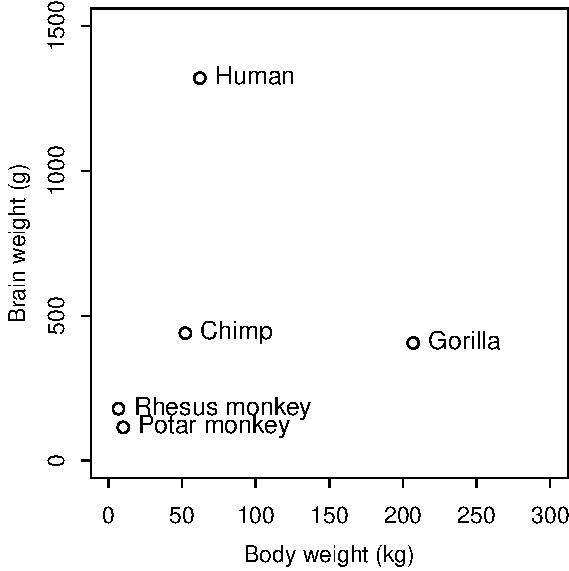
\includegraphics[width=0.47\textwidth]{figs/gph-fig9_1e-1} 

}



\end{knitrout}
\caption{Plot of brain weight against body weight, for selected
primates.}\label{fig:primates}
\end{figure}

\begin{suppfigure}[ht]
\begin{knitrout}
\definecolor{shadecolor}{rgb}{0.969, 0.969, 0.969}\color{fgcolor}\begin{kframe}
\begin{alltt}
\hlkwd{supp9.1}\hlstd{()}
\end{alltt}
\end{kframe}

{\centering 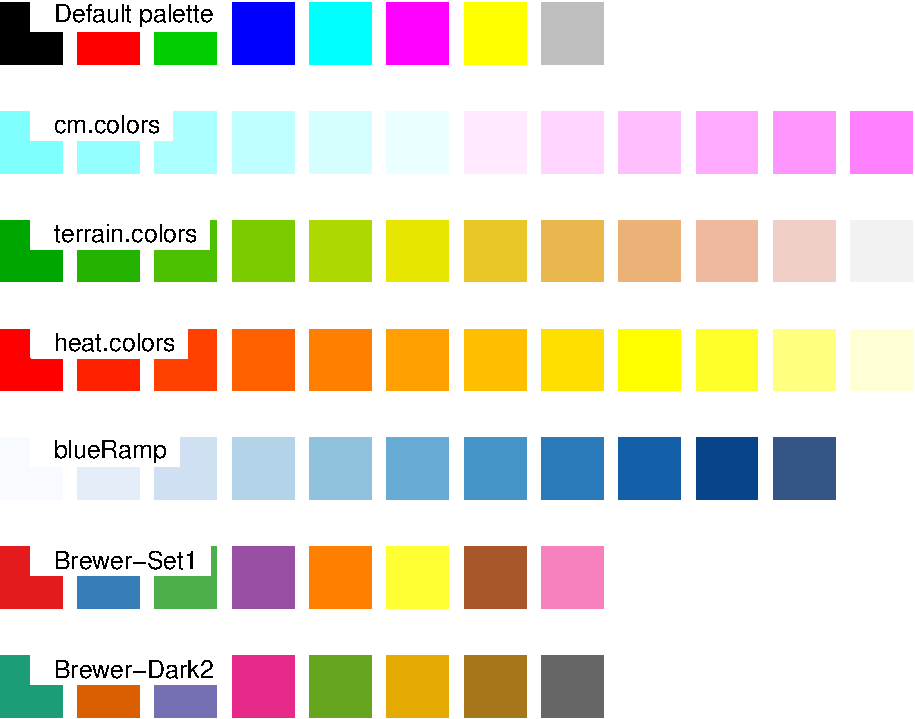
\includegraphics[width=0.75\textwidth]{figs/gph-supp9_1e-1} 

}



\end{knitrout}
\caption{Color palettes.}\label{fig:colpal}
\end{suppfigure}

\begin{figure}[ht]
\begin{knitrout}
\definecolor{shadecolor}{rgb}{0.969, 0.969, 0.969}\color{fgcolor}\begin{kframe}
\begin{alltt}
\hlkwd{fig9.2}\hlstd{()}
\end{alltt}
\end{kframe}

{\centering 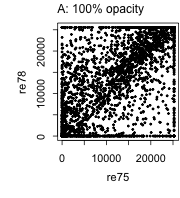
\includegraphics[width=0.32\textwidth]{figs/gph-fig9_2e-1} 
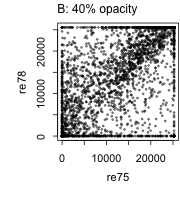
\includegraphics[width=0.32\textwidth]{figs/gph-fig9_2e-2} 
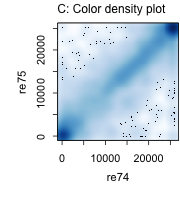
\includegraphics[width=0.32\textwidth]{figs/gph-fig9_2e-3} 

}



\end{knitrout}
\caption{In Panel A, points are plotted with the 100\% opacity, i.e.,
  no transparency. In Panel B, \txtt{alpha=0.4}, i.e., 40\% opacity.
  Panel C uses the function \txtt{smoothScatter()} to show a smoothed
  color density representation of the data.
  \label{fig:alpha}.}
\end{figure}

\begin{figure}[ht]
\begin{knitrout}
\definecolor{shadecolor}{rgb}{0.969, 0.969, 0.969}\color{fgcolor}\begin{kframe}
\begin{alltt}
\hlkwd{par}\hlstd{(}\hlkwc{fig}\hlstd{=}\hlkwd{c}\hlstd{(}\hlnum{0}\hlstd{,}\hlnum{0.265}\hlstd{,} \hlnum{0}\hlstd{,}\hlnum{1}\hlstd{))}
\hlkwd{fig9.3}\hlstd{()}
\hlkwd{mtext}\hlstd{(}\hlkwc{side}\hlstd{=}\hlnum{3}\hlstd{,} \hlkwc{line}\hlstd{=}\hlnum{0.5}\hlstd{,} \hlstr{"A: 1:1 aspect ratio"}\hlstd{,} \hlkwc{adj}\hlstd{=}\hlnum{0}\hlstd{)}
\hlkwd{par}\hlstd{(}\hlkwc{fig}\hlstd{=}\hlkwd{c}\hlstd{(}\hlnum{0.265}\hlstd{,} \hlnum{1}\hlstd{,} \hlnum{0}\hlstd{,}\hlnum{1}\hlstd{),} \hlkwc{new}\hlstd{=}\hlnum{TRUE}\hlstd{)}
\hlkwd{fig9.3}\hlstd{()}
\hlkwd{mtext}\hlstd{(}\hlkwc{side}\hlstd{=}\hlnum{3}\hlstd{,} \hlkwc{line}\hlstd{=}\hlnum{0.5}\hlstd{,} \hlstr{"B: 1:3.5 aspect ratio"}\hlstd{,} \hlkwc{adj}\hlstd{=}\hlnum{0}\hlstd{)}
\end{alltt}
\end{kframe}

{\centering 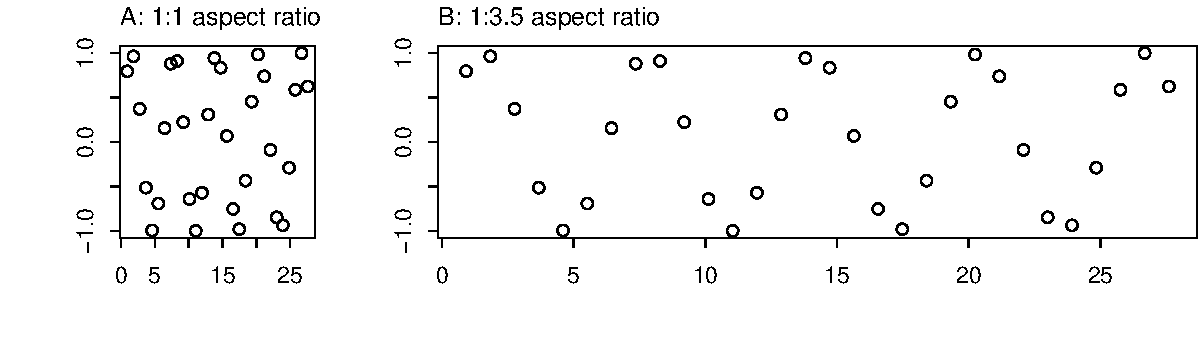
\includegraphics[width=0.9\textwidth]{figs/gph-fig9_3e-1} 

}



\end{knitrout}
\caption{Both figures show the same data, but with very different
  aspect ratios.\label{fig:aspect}}
\end{figure}

\begin{suppfigure}[ht]
\begin{knitrout}
\definecolor{shadecolor}{rgb}{0.969, 0.969, 0.969}\color{fgcolor}\begin{kframe}
\begin{alltt}
\hlkwd{supp9.2}\hlstd{()}
\end{alltt}
\end{kframe}

{\centering 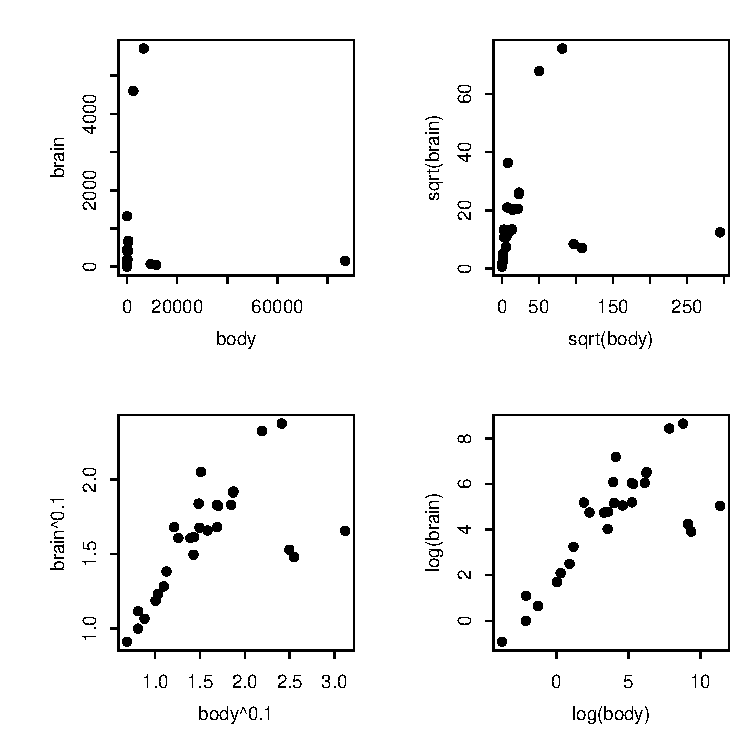
\includegraphics[width=0.8\textwidth]{figs/gph-supp9_2e-1} 

}



\end{knitrout}
\caption{The figure shows a 2 by 2 layout of plots.}
\end{suppfigure}

\begin{figure}[ht]
\begin{knitrout}
\definecolor{shadecolor}{rgb}{0.969, 0.969, 0.969}\color{fgcolor}\begin{kframe}
\begin{alltt}
\hlkwd{fig9.4}\hlstd{()}
\end{alltt}
\end{kframe}

{\centering 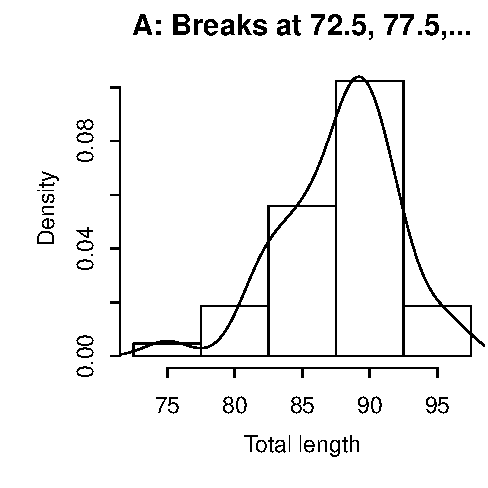
\includegraphics[width=0.47\textwidth]{figs/gph-fig9_4e-1} 
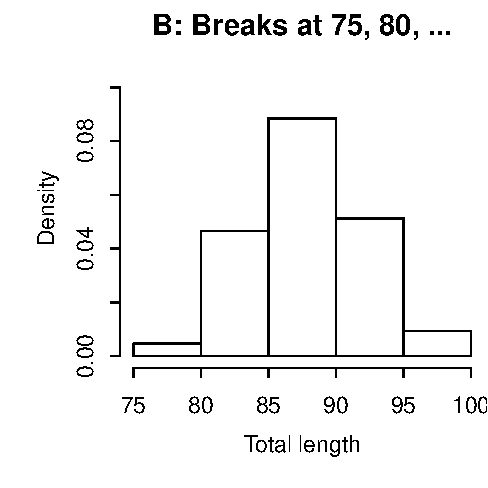
\includegraphics[width=0.47\textwidth]{figs/gph-fig9_4e-2} 

}



\end{knitrout}
\caption{The two panels show the same data, but with a different
choice of breakpoints.\label{fig:densitybreaks}}
\end{figure}

\begin{suppfigure}
\begin{knitrout}
\definecolor{shadecolor}{rgb}{0.969, 0.969, 0.969}\color{fgcolor}\begin{kframe}
\begin{alltt}
\hlkwd{supp9.3}\hlstd{()}
\end{alltt}
\end{kframe}

{\centering 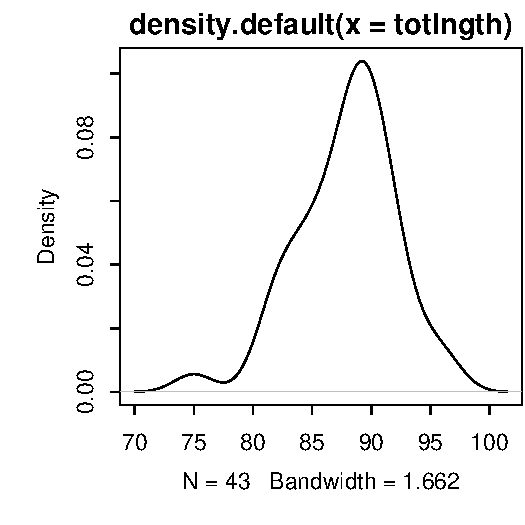
\includegraphics[width=0.47\textwidth]{figs/gph-supp9_3e-1} 

}



\end{knitrout}
\caption{Density plot for lengths of female possums.}
\end{suppfigure}

\clearpage


\begin{figure}[ht]
\begin{knitrout}
\definecolor{shadecolor}{rgb}{0.969, 0.969, 0.969}\color{fgcolor}\begin{kframe}
\begin{alltt}
\hlkwd{fig9.5}\hlstd{()}
\end{alltt}
\end{kframe}

{\centering 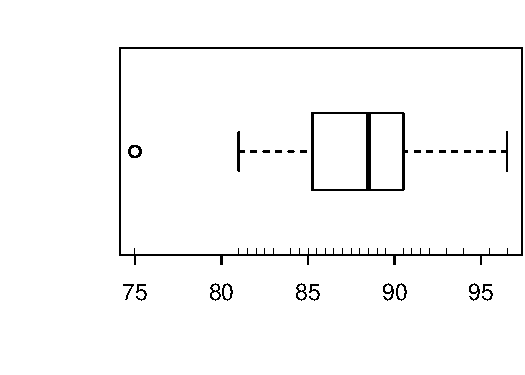
\includegraphics[width=0.42\textwidth]{figs/gph-fig9_5e-1} 

}



\end{knitrout}
\vspace*{-18pt}

\caption{Distribution of lengths of female possums.
The bars (together making up a 'rug') show actual data values.\label{fig:boxrugs}}
\end{figure}

\begin{figure}[ht]
\begin{knitrout}
\definecolor{shadecolor}{rgb}{0.969, 0.969, 0.969}\color{fgcolor}\begin{kframe}
\begin{alltt}
\hlkwd{fig9.6}\hlstd{()}
\end{alltt}
\end{kframe}

{\centering 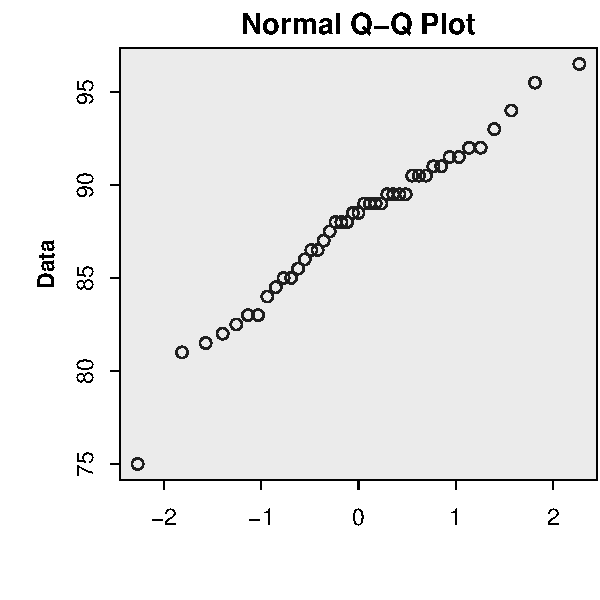
\includegraphics[width=0.24\textwidth]{figs/gph-fig9_6e-1} 
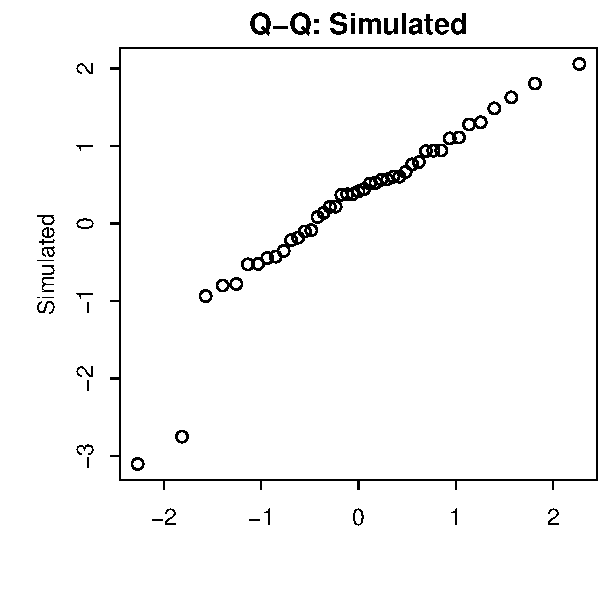
\includegraphics[width=0.24\textwidth]{figs/gph-fig9_6e-2} 
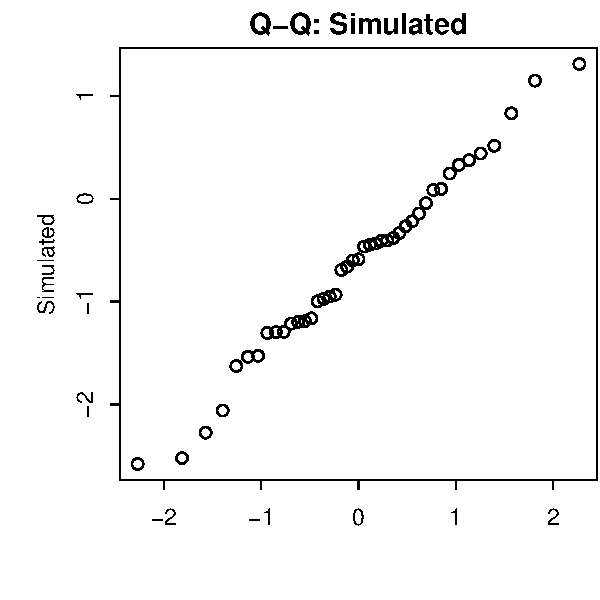
\includegraphics[width=0.24\textwidth]{figs/gph-fig9_6e-3} 
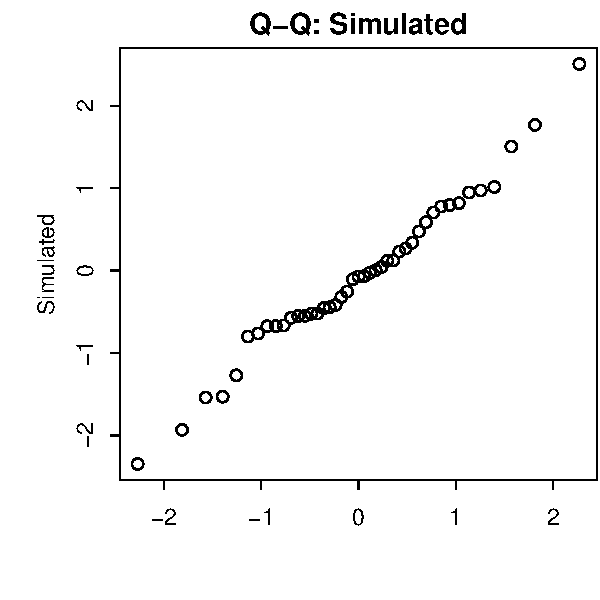
\includegraphics[width=0.24\textwidth]{figs/gph-fig9_6e-4} 
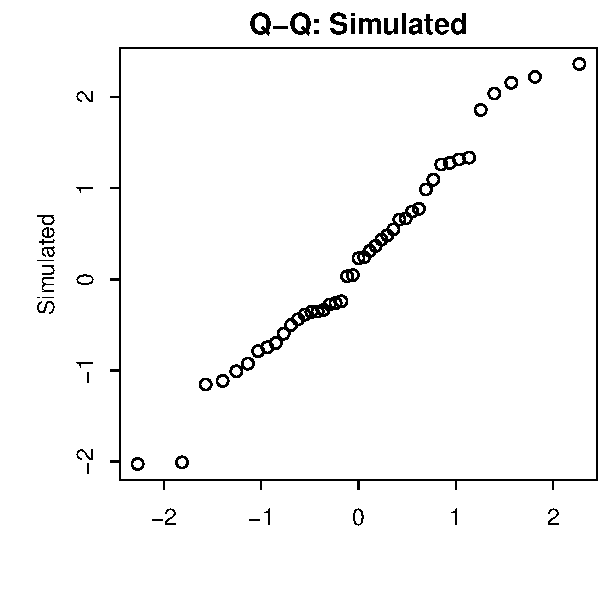
\includegraphics[width=0.24\textwidth]{figs/gph-fig9_6e-5} 
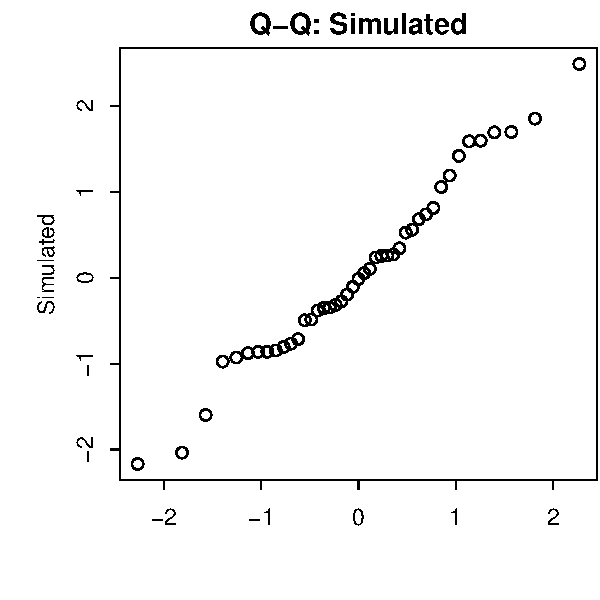
\includegraphics[width=0.24\textwidth]{figs/gph-fig9_6e-6} 
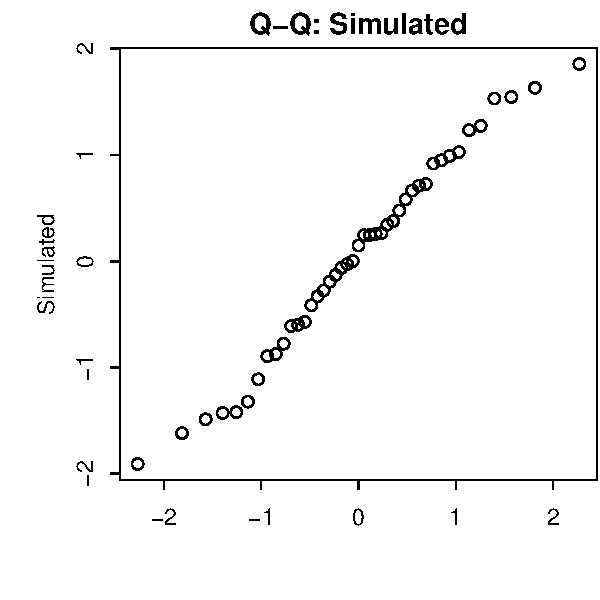
\includegraphics[width=0.24\textwidth]{figs/gph-fig9_6e-7} 
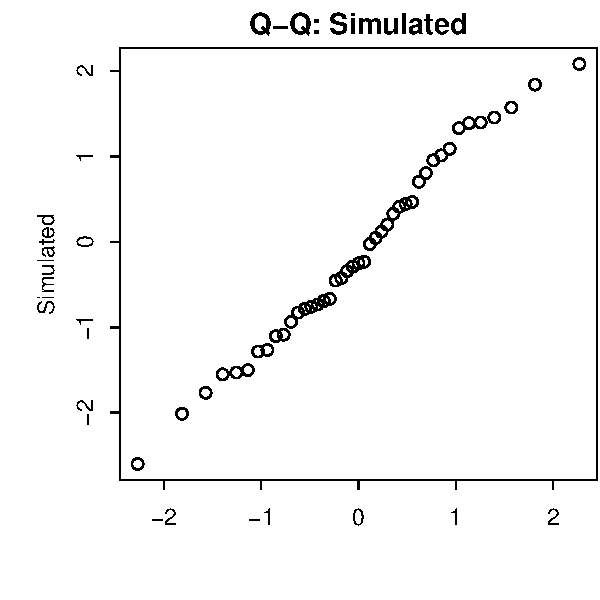
\includegraphics[width=0.24\textwidth]{figs/gph-fig9_6e-8} 

}



\end{knitrout}
\vspace*{-12pt}

      \caption{Normal probability plots. The top left panel shows the 43 lengths
of female possums. Other panels are for independent normal
random samples of size 43.\label{fig:np-plots}}
\end{figure}

\begin{figure}[ht]
\vspace*{-6pt}
\begin{knitrout}
\definecolor{shadecolor}{rgb}{0.969, 0.969, 0.969}\color{fgcolor}\begin{kframe}
\begin{alltt}
\hlkwd{fig9.7}\hlstd{()}
\end{alltt}
\end{kframe}

{\centering 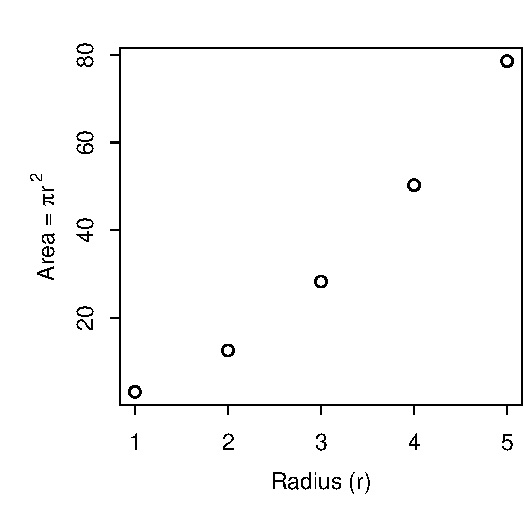
\includegraphics[width=0.47\textwidth]{figs/gph-fig9_7e-1} 

}



\end{knitrout}
\caption{A mathematical expression is included as part of the
  $y$-axis label.\label{fig:area}.}
\end{figure}

\begin{figure}[ht]
\begin{knitrout}
\definecolor{shadecolor}{rgb}{0.969, 0.969, 0.969}\color{fgcolor}\begin{kframe}
\begin{alltt}
\hlkwd{fig9.8}\hlstd{()}
\end{alltt}
\end{kframe}

{\centering 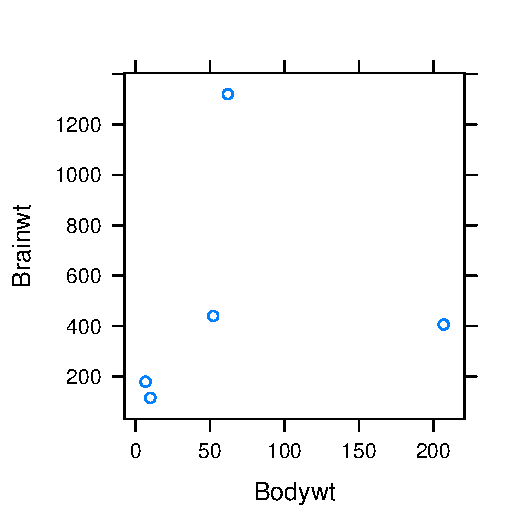
\includegraphics[width=0.47\textwidth]{figs/gph-fig9_8e-1} 

}



\end{knitrout}
\caption{Use of lattice function \txtt{xyplot()} to give a graph.
  \label{fig:lat-gph}}
\end{figure}

\begin{figure}[ht]
\begin{knitrout}
\definecolor{shadecolor}{rgb}{0.969, 0.969, 0.969}\color{fgcolor}\begin{kframe}
\begin{alltt}
\hlkwd{fig9.9}\hlstd{()}
\end{alltt}
\end{kframe}

{\centering 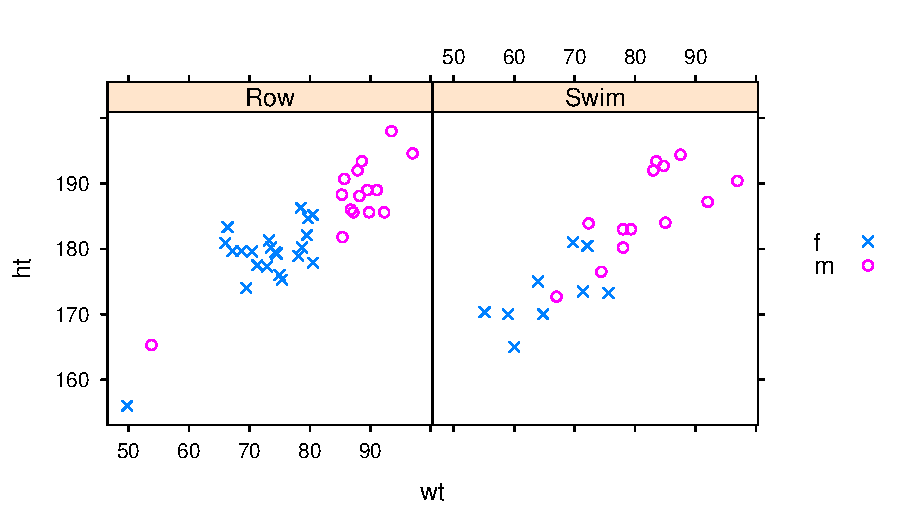
\includegraphics[width=0.8\textwidth]{figs/gph-fig9_9e-1} 

}



\end{knitrout}
\caption{Height (\texttt{ht}) versus Weight (\texttt{wt}), for
        rowers (\texttt{Row}) and swimmers (\texttt{Swim}).
        Different plotting symbols are used to distinguish males from
        females.}\label{fig:lattice-ais}
\end{figure}

\begin{figure}[ht]
\begin{knitrout}
\definecolor{shadecolor}{rgb}{0.969, 0.969, 0.969}\color{fgcolor}\begin{kframe}
\begin{alltt}
\hlkwd{fig9.10}\hlstd{()}
\end{alltt}
\end{kframe}

{\centering 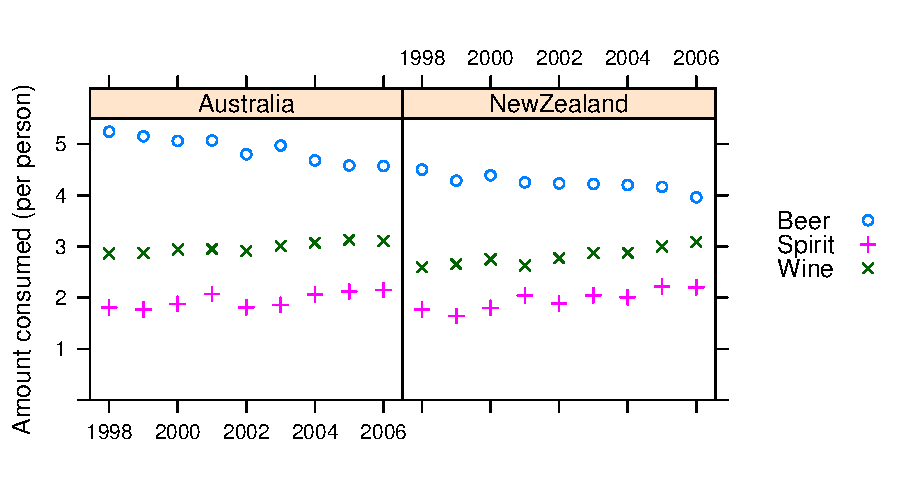
\includegraphics[width=0.8\textwidth]{figs/gph-fig9_10e-1} 

}



\end{knitrout}
\caption{Australian and New Zealand apparent per person annual
  consumption (in liters) of the pure alcohol content of liquor products, for
  1998 to 2006.\label{fig:allgrog}}
\end{figure}

\begin{figure}[ht]
\begin{knitrout}
\definecolor{shadecolor}{rgb}{0.969, 0.969, 0.969}\color{fgcolor}\begin{kframe}
\begin{alltt}
\hlkwd{fig9.11}\hlstd{()}
\end{alltt}
\end{kframe}

{\centering 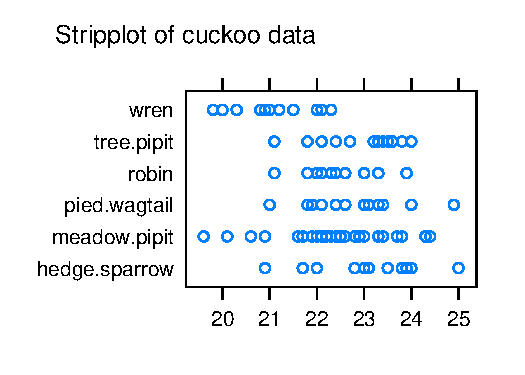
\includegraphics[width=0.47\textwidth]{figs/gph-fig9_11e-1} 

}



\end{knitrout}
\caption{The argument \txtt{legend} has been used to add text,
  supplied as a 'grob'.\label{fig:textGrob}}
\end{figure}

\begin{figure}[ht]
\begin{knitrout}
\definecolor{shadecolor}{rgb}{0.969, 0.969, 0.969}\color{fgcolor}\begin{kframe}
\begin{alltt}
\hlkwd{fig9.12}\hlstd{()}
\end{alltt}
\end{kframe}

{\centering 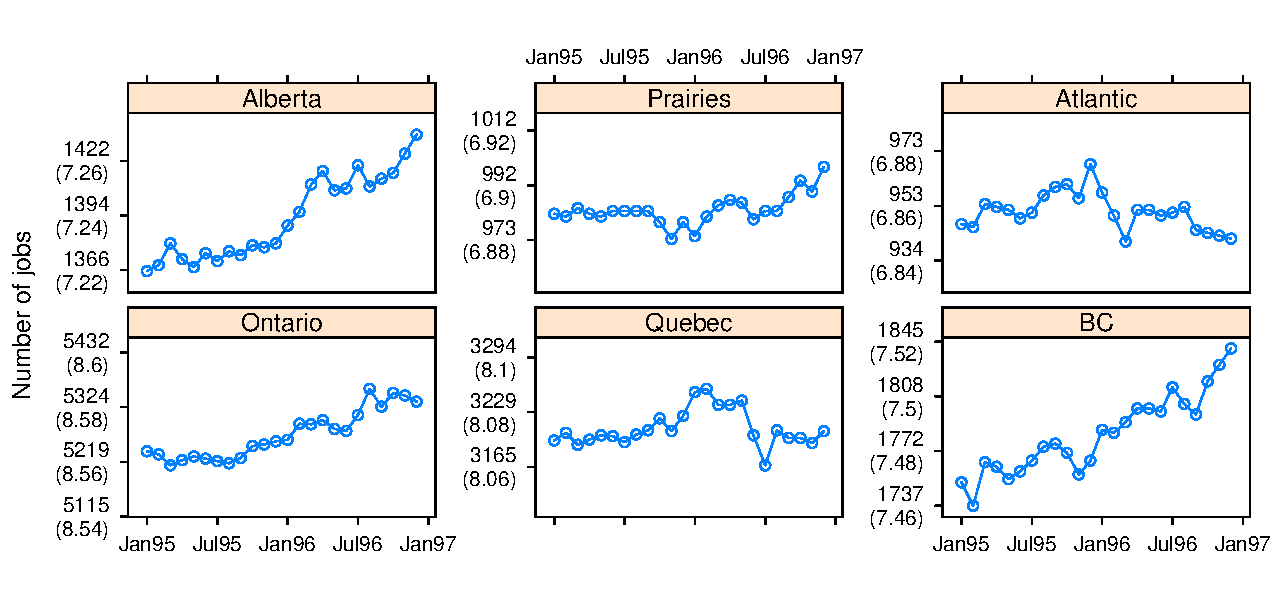
\includegraphics[width=0.97\textwidth]{figs/gph-fig9_12e-1} 

}



\end{knitrout}
\caption{Jobs growth in Canadian provinces, between January 1995
  and December 1996.}\label{fig:jobsplot}
\end{figure}

\begin{figure}[ht]

\caption{A stripplot and a dotplot, side by side for comparison.}
\end{figure}

\begin{figure}[ht]
\begin{knitrout}
\definecolor{shadecolor}{rgb}{0.969, 0.969, 0.969}\color{fgcolor}\begin{kframe}
\begin{alltt}
\hlkwd{fig9.14}\hlstd{()}
\end{alltt}
\end{kframe}

{\centering 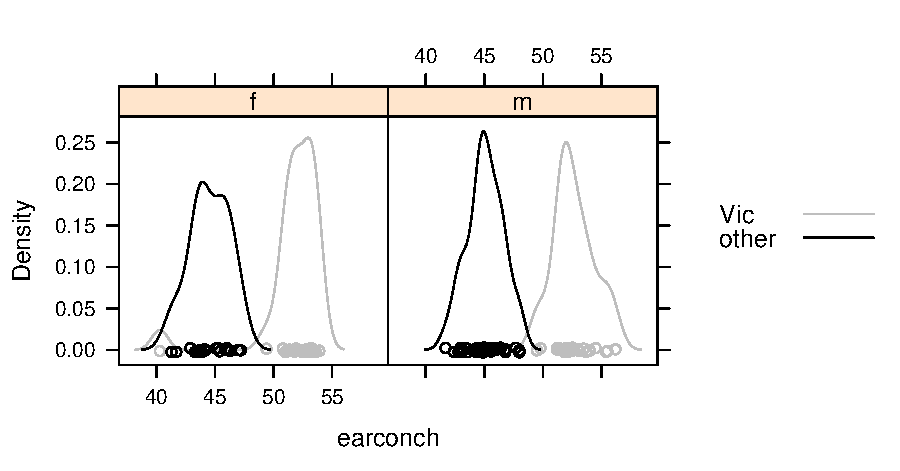
\includegraphics[width=0.8\textwidth]{figs/gph-fig9_14e-1} 

}



\end{knitrout}
\caption{Lattice style density plot comparing possum earconch
    measurements, separately for males and females, between Victorian
    and other populations. Observe that the scatter of data values is
shown along the horizontal axis.}\label{fig:possumdens}
\end{figure}

\begin{figure}[ht]
\begin{knitrout}
\definecolor{shadecolor}{rgb}{0.969, 0.969, 0.969}\color{fgcolor}\begin{kframe}
\begin{alltt}
\hlkwd{fig9.15}\hlstd{()}
\end{alltt}
\end{kframe}

{\centering 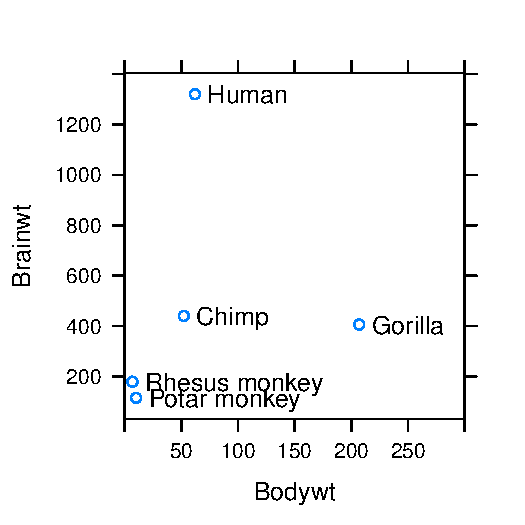
\includegraphics[width=0.47\textwidth]{figs/gph-fig9_15e-1} 

}



\end{knitrout}
\caption{Here, labels have been added to the points. This can be
  done by updating a graph that has the points, by use of a panel
  function that both plots points and and adds labels, or by adding a
  new layer to a graph that shows the points.}\label{fig:layer}
\end{figure}

\addtocounter{figure}{1}

\begin{figure}[ht]
\begin{knitrout}
\definecolor{shadecolor}{rgb}{0.969, 0.969, 0.969}\color{fgcolor}\begin{kframe}
\begin{alltt}
\hlkwd{fig9.17}\hlstd{()}
\end{alltt}
\end{kframe}

{\centering 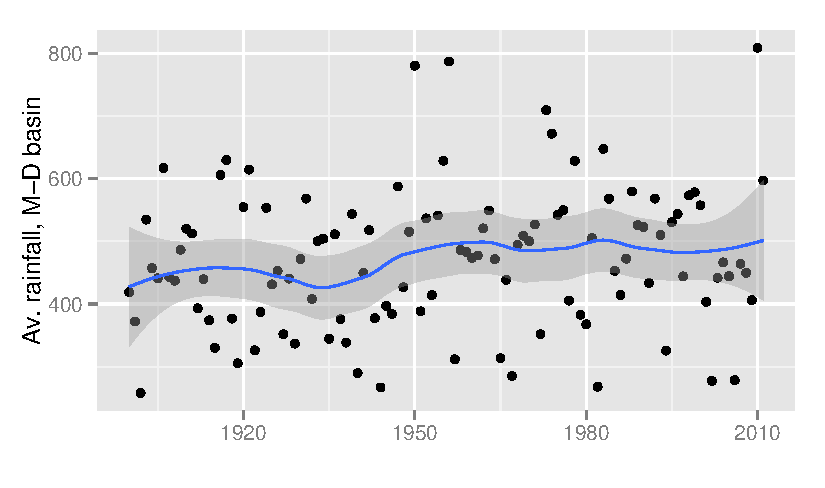
\includegraphics[width=0.8\textwidth]{figs/gph-fig9_17e-1} 

}



\end{knitrout}
\caption{Annual rainfall, from 1901 to 2012, for the Murray-Darling
  basin region of Australia.  The curve is fitted using the default
  loess smoother. The pointwise standard error bands assume that
  errors about the curve are independent; this is unlikely to be
  strictly true. To suppress these bands, specify
  \texttt{se=FALSE}.\label{fig:ggrain}}
\end{figure}

\begin{figure}[ht]
\begin{knitrout}
\definecolor{shadecolor}{rgb}{0.969, 0.969, 0.969}\color{fgcolor}\begin{kframe}
\begin{alltt}
\hlkwd{fig9.18}\hlstd{()}
\end{alltt}
\end{kframe}

{\centering 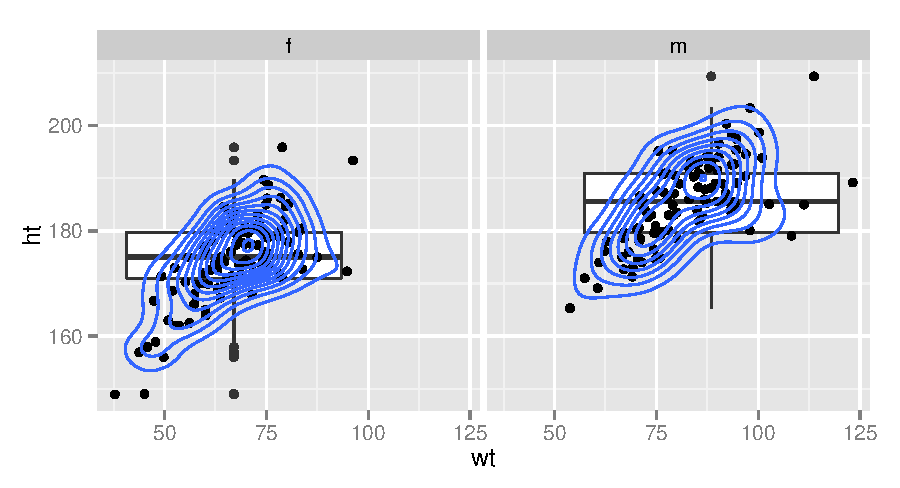
\includegraphics[width=0.8\textwidth]{figs/gph-fig9_18e-1} 

}



\end{knitrout}
\caption{Height versus weight, by sex, for Australian athletes in the
\texttt{ais} data set. Boxplots that show the distributions of heights,
and two-dimensional density contours have been
added.\label{fig:ggais}}

\end{figure}

\begin{suppfigure}
\begin{knitrout}
\definecolor{shadecolor}{rgb}{0.969, 0.969, 0.969}\color{fgcolor}\begin{kframe}
\begin{alltt}
\hlkwd{supp9.4}\hlstd{()}
\end{alltt}
\end{kframe}

{\centering 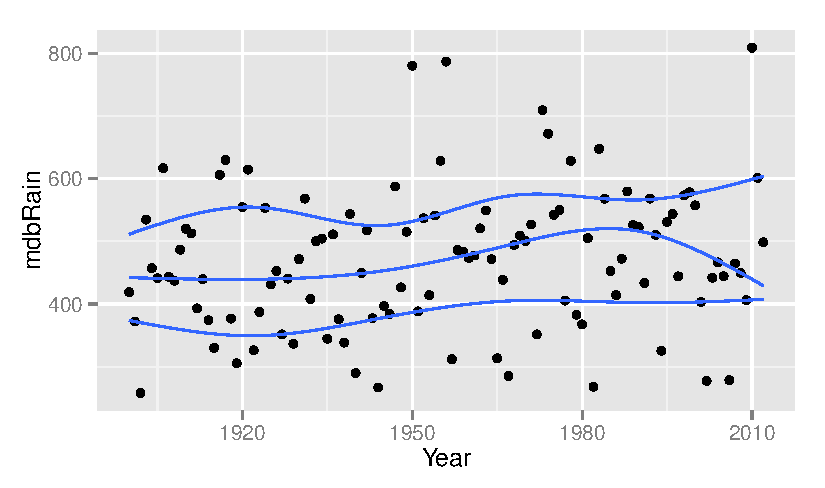
\includegraphics[width=0.8\textwidth]{figs/gph-supp9_4e-1} 

}



\end{knitrout}
\caption{Annual rainfall, from 1901 to 2012, for the Murray-Darling
  basin region of Australia.  Curves that estimate the 20\%, 50\% and 80\%
  quantiles have been fitted.\label{fig:ggrainpc}}
\end{suppfigure}

\begin{figure}[ht]
\begin{knitrout}
\definecolor{shadecolor}{rgb}{0.969, 0.969, 0.969}\color{fgcolor}\begin{kframe}
\begin{alltt}
\hlkwd{fig9.19}\hlstd{()}
\end{alltt}
\end{kframe}

{\centering 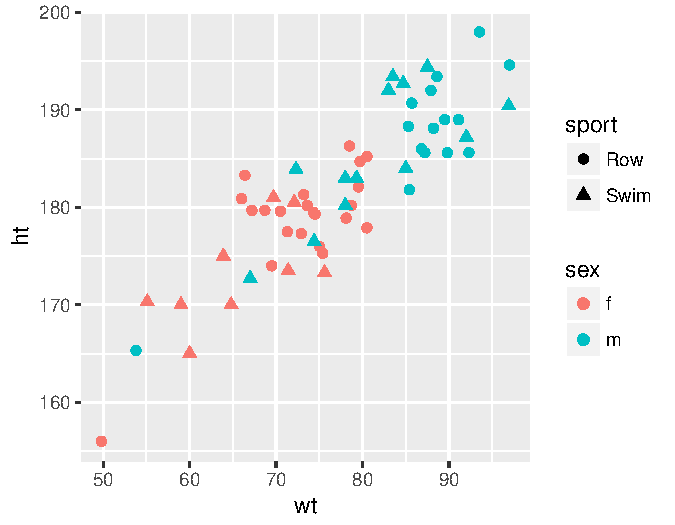
\includegraphics[width=0.8\textwidth]{figs/gph-fig9_19e-1} 

}



\end{knitrout}
\caption{Use \texttt{color} for distinguishing \texttt{sex}es,
\texttt{shape}s for \texttt{sport}s.}\label{fig:colshape}
\end{figure}

\end{document}
